\documentclass[a4paper,11pt,oneside,fleqn,titlepage]{report}

\usepackage{amsmath,amsthm,amssymb}

\usepackage[UKenglish]{babel}

\usepackage{bm}
\usepackage{xcolor}
\usepackage{graphicx}
\usepackage{siunitx}
\sisetup{per-mode=symbol}

\usepackage{booktabs}
\usepackage{caption}

\usepackage{tikz}
\usetikzlibrary{arrows,backgrounds}

\newcommand{\Ncoils}{N_{\textup{coils}}}
\newcommand{\Nturns}{N_{\textup{turns}}}
\newcommand{\Nlayers}{N_{\textup{layers}}}
\newcommand{\npp}{n_{\textup{pp}}}
\newcommand{\nc}{n_{\textup{c}}}
\newcommand{\ncs}{n_{\textup{cs}}}
\newcommand{\Nc}{N_{\textup{c}}}
\newcommand{\Sc}{S_{\textup{c}}}
\newcommand{\Sceq}{S_{\textup{c,eq}}}
\newcommand{\Uw}{U_{\textup{w}}}
\newcommand{\Iw}{I_{\textup{w}}}

\newcommand{\kfill}{k_{\textup{fill}}}
\newcommand{\Jslot}{J_{\textup{slot}}}
\newcommand{\Islot}[1][]{I_{\textup{slot}#1}}
\newcommand{\islot}[1][]{\vec{i}_{\textup{slot}#1}}
\newcommand{\Sslot}{S_{\textup{slot}}}

\newcommand{\eu}{\textrm{e}}
\newcommand{\je}{\textrm{j}}
\newcommand{\thh}{\vartheta}
\newcommand{\thm}{\thh_{\textup{m}}}
\newcommand{\thme}{\thm^{\textup{e}}}
\newcommand{\alphaie}{\alpha_{\textup{i}}^{\textup{e}}}

\newcommand{\sv}[1]{\bm{#1}}
\renewcommand{\vec}[1]{\overline{#1}}

\title{3F --- Framework for \textsc{Femm}}
\author{}

\begin{document}

\begin{titlepage}
\centering

\includegraphics[width=0.5\textwidth]{../more/icon/icon.pdf}
\\[2cm]

\LARGE 3F --- Framework for \textsc{Femm}
\vfill
\end{titlepage}


\tableofcontents

\chapter{Geometry}

\section{Slots}
\makebox[1\textwidth][c]{
\begin{tabular}{ccccccc}
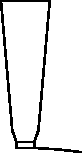
\includegraphics{../examples/slots/squared_slot} &
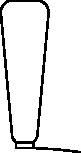
\includegraphics{../examples/slots/rounded_slot} &
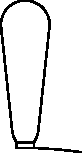
\includegraphics{../examples/slots/round_slot} &
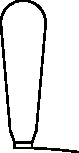
\includegraphics{../examples/slots/semiround_slot} &
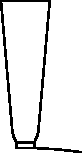
\includegraphics{../examples/slots/roundsemi_slot} &
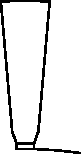
\includegraphics{../examples/slots/semiarc_slot} &
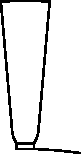
\includegraphics{../examples/slots/roundarc_slot} \\
%
\texttt{squared} &
\texttt{rounded} &
\texttt{round} &
\texttt{semiround} &
\texttt{roundsemi} &
\texttt{semiarc} & 
\texttt{roundarc}
\end{tabular}}
\vspace{1cm}


% Stators
\newpage
\section{Stators}
\begin{tabular}{c}
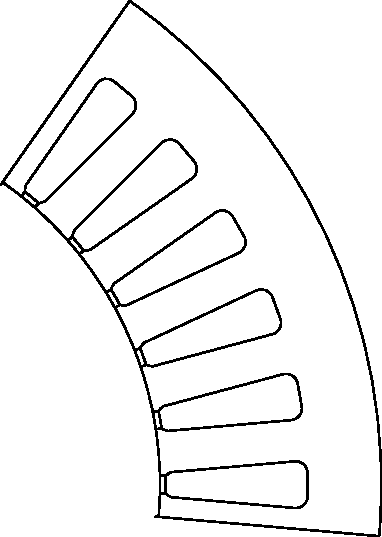
\includegraphics[scale=0.75]{../examples/stators/1pole} 
\\
$ 1 $ \texttt{pole}
\end{tabular}
\vspace{5mm}

\begin{tabular}{c}
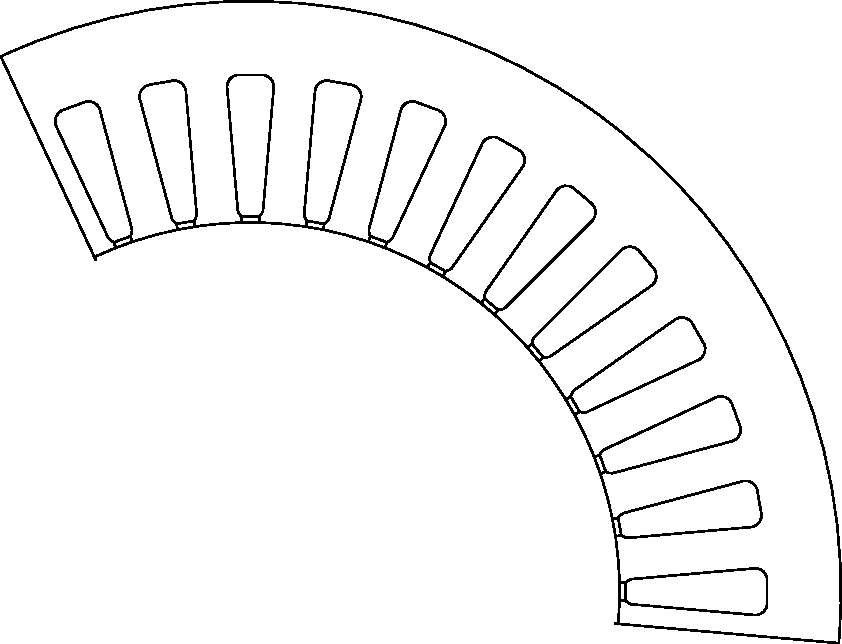
\includegraphics[scale=0.75]{../examples/stators/2pole} 
\\
$ 2 $ \texttt{poles}
\end{tabular}
\vspace{5mm}

\begin{tabular}{c}
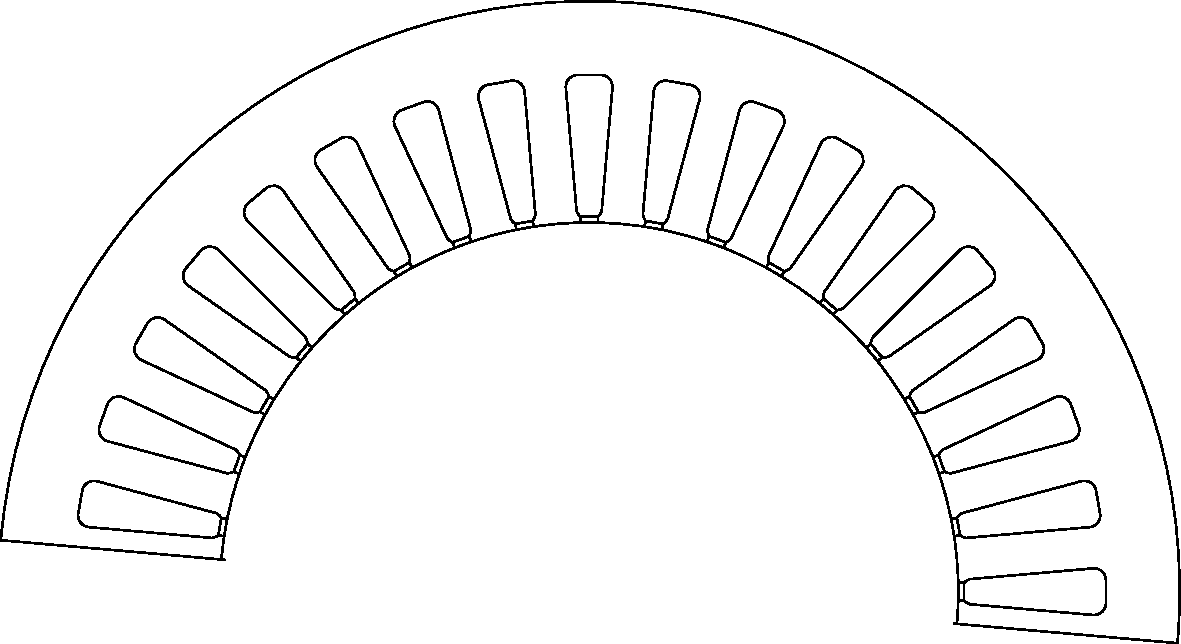
\includegraphics[scale=0.75]{../examples/stators/ppole} 
\\
$ p $ \texttt{poles}
\end{tabular}
\vspace{5mm}

\begin{tabular}{c}
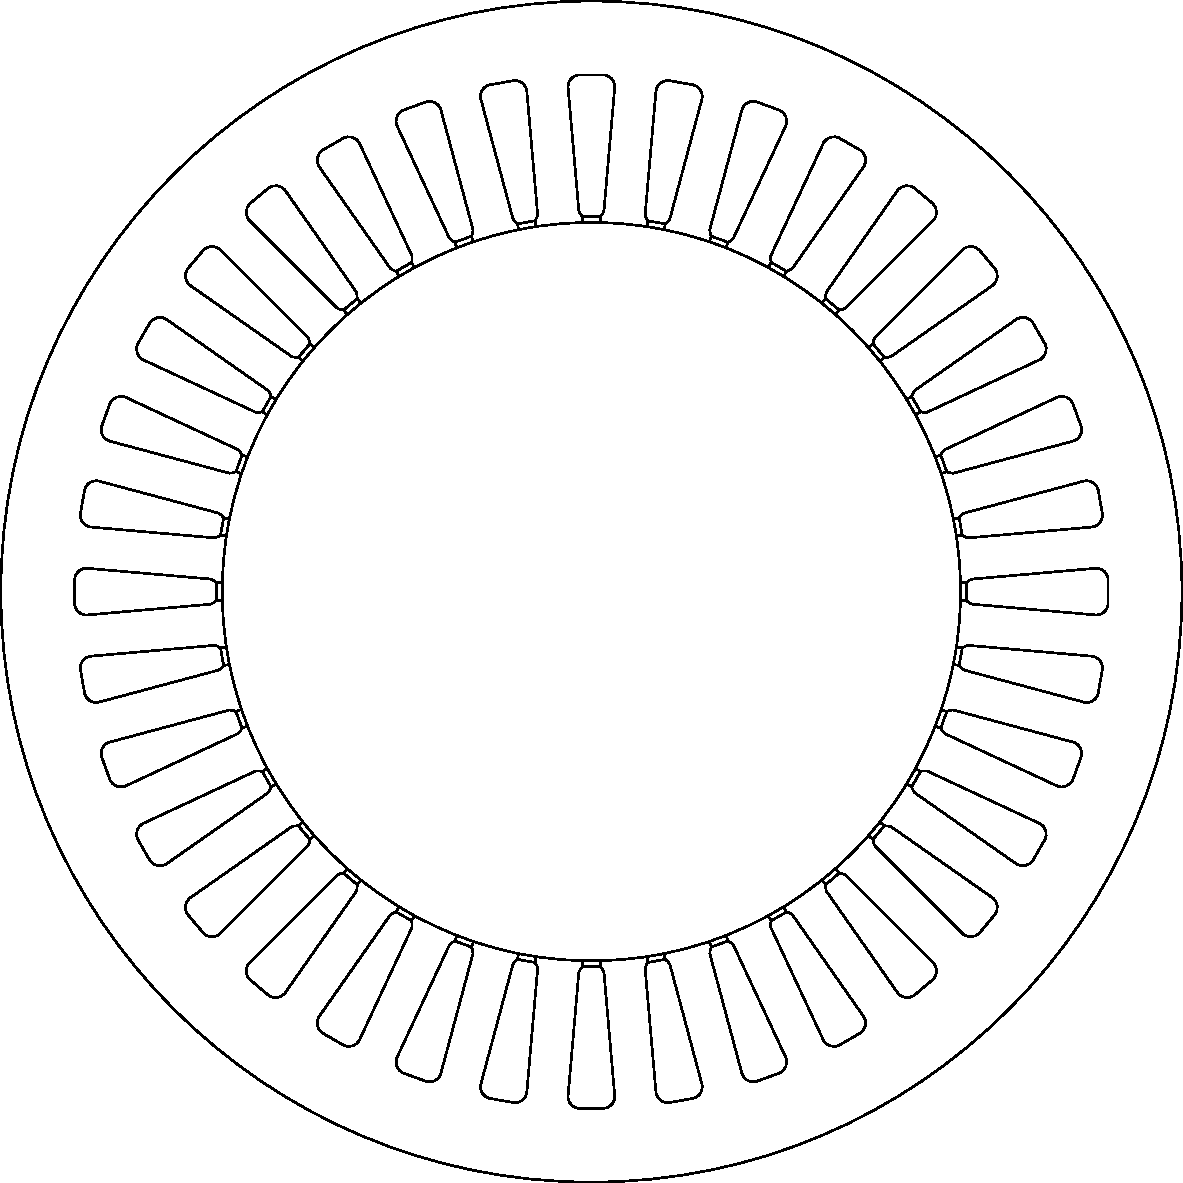
\includegraphics[scale=0.75]{../examples/stators/2ppole}
 
\\
$ 2p $ \texttt{poles}
\end{tabular}



% Magnets
\newpage
\section{SPM Magnets}

\begin{tabular}{c}
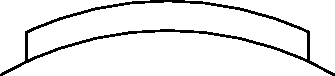
\includegraphics[scale=1]{../examples/magnets/parallel_rect}
\\
\texttt{parallel + rect}
\end{tabular}
\vspace{5mm}

\noindent
\begin{tabular}{c}
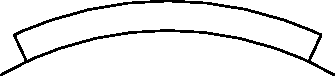
\includegraphics[scale=1]{../examples/magnets/parallel_trapz}
\\
\texttt{parallel + trapz}
\end{tabular}
\vspace{5mm}

\noindent
\begin{tabular}{c}
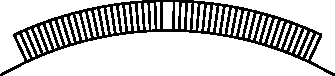
\includegraphics[scale=1]{../examples/magnets/radial_trapz}
\\
\texttt{radial (+ trapz)}
\end{tabular}




% Rotors
\newpage
\section{SPM Rotors}
\begin{tabular}{c}
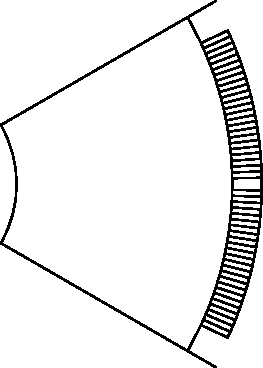
\includegraphics[scale=0.75]{../examples/rotors/1pole} 
\\
$ 1 $ \texttt{pole}
\end{tabular}
\vspace{5mm}

\begin{tabular}{c}
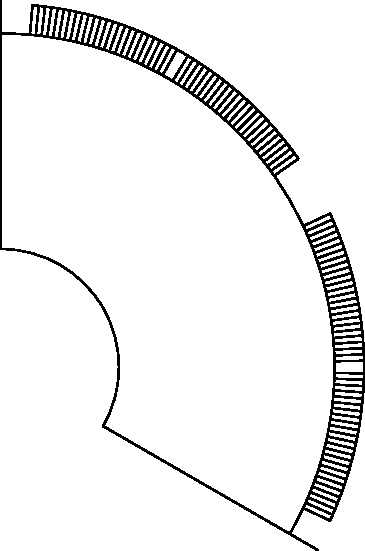
\includegraphics[scale=0.75]{../examples/rotors/2pole} 
\\
$ 2 $ \texttt{poles}
\end{tabular}
\vspace{5mm}

\begin{tabular}{c}
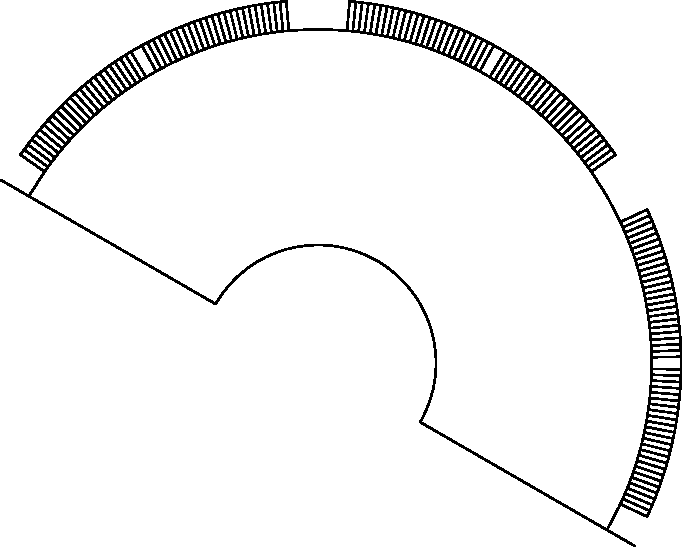
\includegraphics[scale=0.75]{../examples/rotors/ppole} 
\\
$ p $ \texttt{poles}
\end{tabular}
\vspace{5mm}

\begin{tabular}{c}
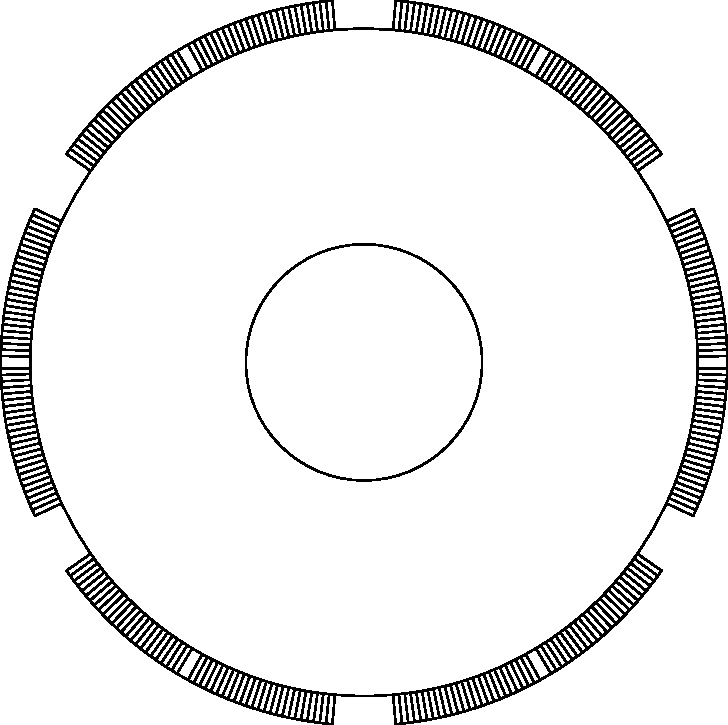
\includegraphics[scale=0.75]{../examples/rotors/2ppole} 
\\
$ 2p $ \texttt{poles}
\end{tabular}






\chapter{Winding}
We will characterise a winding through

\begin{table}[h]
\centering
\begin{tabular}{lll}
\toprule
Name         & Math symbol    & Code symbol 
\\\midrule
%
N. of phases & $ m $          & \texttt{m} 
\\
N. of coils  & $ \Ncoils $ & 
\texttt{coils} \\
N. of turns per coil & $ \Nturns $ & 
\texttt{turns} \\
N. of layers & $ \Nlayers $ & \texttt{layers} \\
N. of parallel paths & $ \npp $ & \texttt{ppath} \\
N. of conductors in slot & $ \nc $ & \texttt{nc} \\
\bottomrule
\end{tabular}
\end{table}

Typically, given a lamination stack with $ Q $ slots
\begin{equation*}
\Ncoils = \frac{Q}{2}\,\Nlayers
\end{equation*}
so if the number of layers is one, the number of coils is 
half the number of slots, given the fact that a coil side 
occupies a full slot.
\begin{equation*}
\nc = \Nlayers\,\Nturns
\end{equation*}
This equation means that in each slot there are $ \nc $ conductors of 
any phase due to the turns in each coil side in each layer.
We bring this number to the equivalent series-connected machine, through the 
number of parallel paths:
\begin{equation*}
\ncs = \frac{\nc}{\npp}
\end{equation*}
This number, $ \ncs $, is related to the complete set of slots, while the 
previous $ \nc $ was related only to a part of them, due to the parallel 
connection of the winding. Thanks to this fact, we can compute the whole number 
of conductors for each phase, through
\begin{equation*}
\Nc = \frac{Q\,\ncs}{m}
\end{equation*}
Therefore the full number of turns for each phase, which will appear in the 
flux linkage, is $ \Nc/2 $. This number is valid for both the real machine and 
the equivalent series-connected one.

Another equivalence that we will use is the wye-equivalence. For both the wye 
and the delta connection of the windings, we will refer to the wye equivalent 
winding. Each winding sustains either the line(-to-line) voltage in the wye 
(delta) connection. 
Therefore
\begin{align*}
\Uw &= \frac{U_{\textup{N}}}{\sqrt{3}} \quad[\si{\volt}]	\qquad \text{delta 
connection} \\[1ex]
\Uw &= U_{\textup{N}} \quad[\si{\volt}]	\qquad \text{wye connection}
\end{align*}
In this way we can obtain the winding current directly from the power
\[
\Iw = \frac{P}{3 \Uw\cos\varphi} \quad[\si{\ampere}]
\]
and use it as the design current for the winding itself. In fact, if each turn 
is made by some wires with a full section $ \Sc $, we will refer to the 
equivalent turn section
\[
\Sceq = \npp \Sc \quad [\si{\milli\meter\squared}]
\]
which sees the complete winding current, giving the current density
\[
J = \frac{\Iw}{\Sceq} \quad [\si{\ampere\per\milli\meter\squared}]
\]
It is important to highlight that this current density is the conductor's one, 
while the slot current density is given by
\[
\Jslot = \kfill J \quad [\si{\ampere\per\milli\meter\squared}]
\]
where the fill factor, $ \kfill $, represents the ratio between the actual 
conductor area in the slot and the slot section.
Depending on the starting point, one can find the rms current in the slot 
through
\[
\Islot = \Jslot \Sslot = \ncs \Iw \quad[\si{\ampere}]
\]



\section{Space vector}
Given an $ m $-phase winding symmetrically distributed, we can associate its 
currents to a single complex-valued variable, the \emph{space vector}, which 
represents the equivalent primitive two-phase winding, with axes $ \alpha $ and 
$ \beta $. Thus
\[
\sv{i}_{\alpha\beta} = \frac{2}{m}\,\left[ 
i_a + i_b\,\eu^{\,\je\frac{2\pi}{m}} + i_c\,\eu^{\,\je\frac{4\pi}{m}} + \ldots
+ i_m\,\eu^{\,\je\frac{(m-1)2\pi}{m}}
\right] = \sv{i}^s
\]
If we want to get the space vector in the synchronous reference frame, it is 
simply
\[
\sv{i}^r = \sv{i}^s\,\eu^{-\je\thme}
\]
Therefore we can directly relate the $ dq $-current to the 
$ m $ phase currents:%
\footnote{The adopted convention is the following
\[
T\text{ransformation}_{\text{from}}^{\text{to}} \qquad
U\text{antitransformation}_{\text{from}}^{\text{to}}
\]%
}
\begin{align*}
\vec{i}_{\textup{s}} \xrightarrow{T_{ab\cdots m}^{dq}} 
\sv{i}^r
\end{align*}


\section{Slot matrix}
The slot matrix is a useful tool for the correct and rapid 
assignment of currents in the slots. In fact it directly 
relates phase and slot currents, through
\[
\vec{i}_{\textup{s}} \xrightarrow{\;K\;} 
\vec{i}_{\textup{slot}}
\]
This relationships is missing just the number of series 
conductor per slot. So
\[
\vec{i}_{\textup{slot}} = \ncs K \, \vec{i}_s
\]


\section{Sinusoidal dq control}
For synchronous machines, this is the typical control 
implemented. A reference current, which comes from the 
speed loop, is imposed. Usually the control is executed in 
the $ dq $-reference frame, therefore we start from
\[
\sv{i}^r = i_d + \je i_q = |\sv{i}|\,\eu^{\,\je\alphaie}
\]
Then we transform it in the $ \alpha\beta $-reference frame 
and finally we get the phase currents:%
\footnote{%
In the code the transformations made available are
\texttt{dq2ab} and \texttt{U}, which is the one from $ 
\alpha\beta $ to $ abc\cdots m $.
}
\[
\vec{i}_{\textup{s}} = U_{s}^{ab\cdots m}\sv{i}^s = 
U_{s}^{ab\cdots m} 
U_{r}^{s}\,\sv{i}^r = U_{r}^{ab\cdots m}\,\sv{i}^r
\]
%
From here, the slot currents are simply
\[
\islot = \ncs K\,\vec{i}_{\textup{s}} = \ncs 
K\,U_{r}^{ab\cdots 
m}\,\sv{i}^r
\]


\section{Trapezoidal control}
This control is typical of BLDC drives.
In the trapezoidal control the currents would ideally 
assume just three values:
\[
\{ +I_{\textup{DC}},0,-I_{\textup{DC}} \}
\]
while the current absorbed from the DC-bus is constant.
Only two phases are active simultaneously, while the third 
one is kept off. Taking half the DC-bus voltage as the 
reference, the voltages assume just three values too:
\[
\{ +V_{\textup{DC}}/2,0,-V_{\textup{DC}}/2 \}
\]
The complete number of possible states is the double ($ +/- 
$) of all the grouping of the phases ($ m $) by two:
\[
\text{\# of states} = 2\,\binom{m}{2} = m\,(m - 1)
\]
Consider a three-phase machine for instance. The supply 
states can be
\[
\begin{array}{rcccc}
\text{state 6}& \quad &   +   &   -   &   0   \\
\text{state 1}& \quad &   +   &   0   &   -   \\
\text{state 2}& \quad &   0   &   +   &   -   \\
\text{state 3}& \quad &   -   &   +   &   0   \\
\text{state 4}& \quad &   -   &   0   &   +   \\
\text{state 5}& \quad &   0   &   -   &   +   
\end{array}
\]

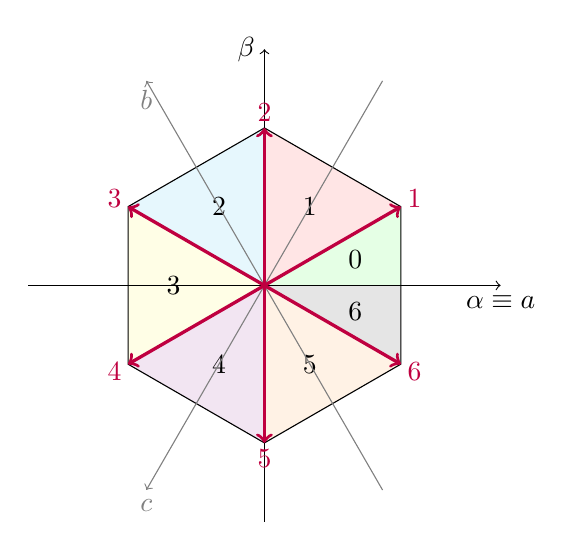
\begin{tikzpicture}
\def \L {20mm};

% draw axis
\draw[->] (-1.5*\L,0) -- (1.5*\L,0) node[anchor=north] {$ 
\alpha \equiv a $} ;
\draw[->] (0,-1.5*\L) -- (0,1.5*\L) node[anchor=east] {$ 
\beta $} ;
\draw[->,gray] (120+180:1.5*\L) -- (120:1.5*\L) 
node[anchor=north] {$ b $} ;
\draw[->,gray] (240+180:1.5*\L) -- (240:1.5*\L) 
node[anchor=north] {$ c $} ;

\coordinate (0) at (0,0);

\foreach \i in {1,2,...,6}
{
\coordinate (\i) at ({30 + (\i-1)*60}:\L);
\coordinate (s\i) at ({30 + (\i-1)*60}:1.1*\L);
\draw[->,purple,very thick] (0) -- (\i) ;
\node[purple] at (s\i) {\i} ;
}

\begin{scope}[on background layer]
\coordinate (a) at ({sqrt(3)/2*\L},0) ;
\fill[green!10] (0) -- (a) -- (1) -- cycle ;
\fill[red!10] (0) -- (1) -- (2) -- cycle ;
\fill[cyan!10] (0) -- (2) -- (3) -- cycle ;
\fill[yellow!10] (0) -- (3) -- (4) -- cycle ;
\fill[violet!10] (0) -- (4) -- (5) -- cycle ;
\fill[orange!10] (0) -- (5) -- (6) -- cycle ;
\fill[black!10] (0) -- (6) -- (a) -- cycle ;

\node at (barycentric cs:0=1,a=1,1=1) {0};
\foreach \i in {1,...,5}
{
\pgfmathsetmacro \j {int(\i+1)};
\node at (barycentric cs:0=1,\i=1,\j=1) {\i};
}
\node at (barycentric cs:0=1,6=1,a=1) {6};

\draw (1) -- (2) --(3) -- (4) -- (5) -- (6) -- cycle;
\end{scope}

\end{tikzpicture}

\end{document}